\subsection{Summary of the standard fitting algorithm}

The standard FFT-based 3D fitting algorithm operates according to
the workflow shown in Figure \ref{fig:CartesianFFT} \cite{Katchalski-Katzir1992,Gabb1997,Chacon2002}. The input of
this algorithm is a protein atomic structure determined experimentally
by, e.g., X-ray crystallography or nuclear magnetic resonance (NMR)
experiments. Another input is an experimental EDM
determined by means of, e.g., cryo-EM.
First, the algorithm decomposes
the experimental EDM into the Fourier basis using the fast Fourier
transform algorithm. Then, it rotates the protein
structure to a certain orientation $\mathbf{r}$ and decomposes the electron density of the
rotated structure into the Fourier basis. 

\begin{figure}[ht!]
\label{fig:CartesianFFT}
\caption[Flowchart of the standard fitting algorithm]{Flowchart of the standard fitting algorithm based on the Fourier correlations.
Green blocks correspond to the operations in the Fourier space.}
\includegraphics[width=1\textwidth]{Hermite/Fig/figure1}
\end{figure}

%
The electron density is typically computed as a sum of Gaussians centred on non-hydrogen atoms of the protein. 
%
Afterwards, the algorithm exhaustively
explores translational degrees of freedom of the rotated protein with
respect to the EDM. For every translation $\mathbf{t}$,
it determines the corresponding score, which is usually given by the
correlation between the two densities. This procedure is equivalent
to computing the convolution of two functions, 
\begin{equation}
\textrm{CCF}(\mathbf{r}, \mathbf{t})=\int d\mathbf{x}\, f(\mathbf{r},\mathbf{x}-\mathbf{t})g(\mathbf{x}),\label{eq:convolution}
\end{equation}
where $f(\mathbf{r},\mathbf{x-t})$ is the density of the protein rotated by $\mathbf{r}$ and translated by $\mathbf{t}$,
and $g(\mathbf{x})$ is the experimental electron density map. 
To speed up this step, the algorithm
computes the values of the Fourier transform of the CCF
for all translational degrees of freedom at once, using the convolution
theorem. Finally, the algorithm computes the inverse Fourier transform
(IFT) of the convolution, generates a new rotation of the protein
structure, and returns to the second step. This procedure is repeated
until all rotational degrees of freedom of the protein with respect
to the EDM are explored (see Fig. \ref{fig:CartesianFFT}). The solution
of the fitting problem is then given by $(\mathbf{r}_{max},\mathbf{t}_{max})=\mbox{argmax}_{\mathbf{r}, \mathbf{t}}\left\{ \textrm{CCF}(\mathbf{r}, \mathbf{t})\right\} $.


The bottleneck of the standard algorithm is 
the re-projection of the protein electron density into the Fourier space after each rotation.
%
%\blue{[Probably, we can stress this part more, as Lunin suggested]}
To overcome it, we propose to
encode the electron density of the protein structure in the orthogonal
Hermite basis, prior to performing the rotational search. This
allows to speed up the projection of the protein density into the
Fourier space. 
Since only the members of the Fourier family of linear transforms
can replace $O(N^2)$ operations of a convolution in a time domain by $O(N)$ operations in a frequency domain \cite{stone:1998}, we still need to
perform the convolution in the Fourier space.
%
Figure \ref{fig:FourierFitting} shows the workflow of the proposed algorithm.
Computational complexity of this algorithm is listed in Table \ref{table:FourierFitComp}.

\begin{figure}[H]
\label{fig:FourierFitting}
\includegraphics[width=1\textwidth]{Hermite/Fig/figure2}
\caption[Flowchart of HermiteFit]{Flowchart of HermiteFit, the new fitting algorithm based on the Hermite expansions.
Green blocks correspond to the operations in the Fourier space. Blue
blocks correspond to the operations in the Hermite space.}
\end{figure}

\begin{table}
\resizebox{\textwidth}{!}{
\begin{tabular}{|c|c|c|}
\hline 
Operation & Complexity & Loop multiplier \tabularnewline
\hline 
\hline 
Decomposition of the step function & 
$O(M^{3}\mbox{log}M^{3})$ & \multirow{4}{*}{1} \tabularnewline
\cline{1-2} 
Decomposition of the Gaussian & $O(N_{atoms}N^{3})$ & \tabularnewline 
\cline{1-2} 
Construction of the rotation matrix & $O(N_{rot}N^{4})$ & \tabularnewline
\hline  
Rotation & $O(N^{4})$ & \multirow{4}{*}{$N_{rot}$}\tabularnewline
\cline{1-2} 
Evaluation of the Hermite series & $O(M^{3}\cdot N+M^{2}\cdot N^{2}+M\cdot N^{3})$ & \tabularnewline
\cline{1-2} 
Multiplication & $O(M^{3})$ & \tabularnewline 
\cline{1-2} 
Inverse Fourier Transform & $O(M^{3}\mbox{log}M^{3})$ & \tabularnewline
\hline 
\end{tabular}
}
\medskip
\caption[Complexity of the Hermite fitting algorithm]{ Complexity of the Hermite fitting algorithm. Here, $M$ denotes
the order of the Fourier decomposition; 
$N$ is the order
of the Hermite decomposition; $N_{atoms}$ is the number of atoms in the
protein; $N_{rot}$ -- the number of rotations to be sampled.}
\label{table:FourierFitComp}
\end{table}

\subsection{Hermite functions}


Orthogonal Hermite function of order $n$ is defined as:
%
\begin{equation}
\psi_{n}(x;\lambda)=\frac{\sqrt{\lambda}}{\sqrt{2^{n}n!\sqrt{\pi}}}\exp(-\frac{\lambda^{2}x^{2}}{2})H_{n}(\lambda x),\label{eq:hermiteFunction}
\end{equation}
where $H_{n}(x)$ is the Hermite polynomial and $\lambda$ is the
scaling parameter. 
In Fig. \ref{fig:HermitePic} we show several orthogonal Hermite functions of
different orders with different parameters $\lambda$.
These functions form an orthonormal basis set in $L^2 \left( \mathbb{R} \right)$. A 1D function
$f(x)$ decomposed into the set of 1D Hermite functions up to an
order $N$ reads 
%
\begin{equation}
f(x)=\sum_{i=0}^{N}\hat{f}_{i}\psi_{i}(x;\lambda)\label{eq:decomposition}
\end{equation}
Here, $\hat{f}_{i}$ are the decomposition coefficients, which can
be determined from the orthogonality of the basis functions $\psi_{i}(x;\lambda)$.
Decomposition in Eq. \ref{eq:decomposition} is called the \emph{band-limited
decomposition} with $\psi_{i}(x;\lambda)$ basis functions. To decompose
the EDM and the protein structures, we employ the 3D Hermite functions:
%
\begin{equation}
\psi_{n,l,m}(x,y,z;\lambda)=\psi_{n}(x;\lambda)\psi_{l}(y;\lambda)\psi_{m}(z;\lambda),
\end{equation}
which form an orthonormal basis set in $L^2 \left( \mathbb{R}^3 \right)$. A function $f(x,y,z)$
represented as a band-limited expansion in this basis reads
%
\begin{equation}
f(x,y,z)=\sum_{i=0}^{N}\sum_{j=0}^{N-i}\sum_{k=0}^{N-i-j}\hat{f}_{i,j,k}\psi_{i,j,k}(x,y,z;\lambda)\label{eq:HermiteExpansion3D}
\end{equation}


\begin{figure}[H]
 \label{fig:HermitePic}
\begin{centering}
\includegraphics[width=1\textwidth]{Hermite/Fig/figure3}
\end{centering}
\caption[Hermite functions examples]{Left: 1D Hermite functions of order six for three different scaling
parameters $\lambda$. Right: 1D Hermite functions of two different
orders for the scaling parameter $\lambda=1$.}
\end{figure}

Figure \ref{fig:HermiteSin} shows that Hermite functions are very similar to the cosine functions near the coordinate axis origin. 

\begin{figure}[H]
 \label{fig:HermiteSin}
\begin{centering}
\includegraphics[width=1\textwidth]{Hermite/Fig/H50}
\end{centering}
\caption[Hermite functions and sine function]{Hermite function of the order 50 (solid line) and cosine function with the frequency equal to 50 (dashed line).}
\end{figure}

\subsection{Decomposition of electron densities into the orthogonal Hermite basis}
One of the advantages of the orthogonal Hermite basis is that we can
derive the exact analytical expression for the decomposition coefficients
of a molecular structure. This allows to rapidly obtain the exact
decompositions without costly numerical integration over the 3D space.
In our algorithm, the electron density of the protein ($f(x)$ in Eq. \ref{eq:convolution}, upon which rotation and translation operators act) 
is expanded in the Hermite basis using the Gaussian model.
More precisely, we model the electron density of a single atom in the molecular
structure as a Gaussian centred at the atomic position $\mathbf{r}_{0}^{(i)}$
with the squared variance equal to $\alpha^{2}/2$. Then, the electron
density of the whole molecular structure is given by the following
sum:
%
\begin{equation}
M(\mathbf{r})=\sum_{i=1}^{N_{atoms}}e^{-|\mathbf{r}-\mathbf{r}_{0}^{(i)}|^{2}/\alpha^{2}},\label{eq:protein_density}
\end{equation}
where $\mathbf{r}_{0}^{(i)}$ is the position of the $i$-th atom,
$\alpha/\sqrt{2}$ is the variance of the Gaussian distribution, and
$\mathbf{r}=(x,\, y,\, z)\in \mathbb{R}^{3}$ is the sampling volume. 
Normally, each Gaussian should be weighted with a coefficient corresponding to electron distribution of a particular atom. However, we omit the weights in our approximation.
In the section \ref{Sec: Shifted Gaussian expansion}, we provide analytical expressions (Eqs. \ref{eq:From1DTo3DCoeffs} and \ref{eq:Gaussian1DDecCoefs})
for the decomposition coefficients of $M(\mathbf{r})$ in the 1D and
the 3D cases.

\subsection{Shifted Gaussian expansion}
\label{Sec: Shifted Gaussian expansion}

Here we provide the derivation of the expansion coefficients of a
shifted Gaussian of the following form:
%
\begin{equation}
g(\mathbf{r})=e^{-\frac{|\mathbf{r}-\mathbf{r}_{0}|^{2}}{\alpha^{2}}}
\end{equation}
into the orthogonal Hermite basis. The well known property of this
basis (as well as of any orthogonal basis) is the following:
%
\begin{eqnarray}
\mbox{if }f(x,y,z) & = & f^{(1)}(x)f^{(2)}(y)f^{(3)}(z)\nonumber \\
\mbox{and }f^{(k)}(t) & = & \sum_{i=0}^{N}\hat{f}_{i}^{(k)}\psi_{i}(t;\lambda)\nonumber \\
 & \mbox{then}\nonumber \\
\hat{f}_{i,j,k} & = & \hat{f}_{i}^{(1)}\hat{f}_{j}^{(2)}\hat{f}_{k}^{(3)}\label{eq:From1DTo3DCoeffs}
\end{eqnarray}
First, we derive the decomposition of a 1D Gaussian into the 1D orthogonal
Hermite basis. Then, using property (\ref{eq:From1DTo3DCoeffs})
we obtain the decomposition of a 3D Gaussian into the 3D orthogonal
Hermite basis.
%
More specifically, the 1D Gaussian function reads as:
%
\begin{equation}
g(x)=e^{-\frac{(x-\xi)^{2}}{\alpha^{2}}}
\end{equation}
Its decomposition coefficients are equal to:
%
\begin{eqnarray}
\hat{g}_{n}(\xi;\lambda,\alpha) = \int\, g(x)\psi_{n}(x;\lambda)\, dx =  \nonumber \\ 
\frac{n!\sqrt{\lambda}e^{-\frac{\xi^{2}}{\alpha^{2}}\left(1-\frac{1}{\alpha^{2}\beta^{2}}\right)}}{\sqrt{2^{n}n!\sqrt{\pi}}} \sum_{m=0}^{[\frac{n}{2}]}\frac{(-1)^{m}}{m!(n-2m)!}  \nonumber \\ 
\int e^{-\beta^{2}\left(x-\frac{\xi}{\alpha^{2}\beta^{2}}\right)^{2}} (2\lambda(x-\frac{\xi}{\alpha^{2}\beta^{2}})+\frac{2\lambda\xi}{\alpha^{2}\beta^{2}})^{n-2m}dx   
,\end{eqnarray}
where $\beta^{2}=\frac{\lambda^{2}}{2}+\frac{1}{\alpha^{2}}$. From now on we will, for brevity, write $\hat{g}_{n}$ instead of
$\hat{g}_{n}(\xi;\lambda,\alpha)$. Changing the variables
$t=x-\frac{\xi}{\alpha^{2}\beta^{2}}$ and denoting $a=\frac{\xi}{\alpha^{2}\beta^{2}}$,
we obtain: 
%
\begin{eqnarray}
\hat{g}_{n} = \frac{n!\sqrt{\lambda}e^{-\frac{\xi^{2}}{\alpha^{2}}\left(1-\frac{1}{\beta^{2}}\right)}}{\sqrt{2^{n}n!\sqrt{\pi}}} \sum_{m=0}^{[\frac{n}{2}]}\frac{(-1)^{m}\left(2\lambda\right)^{n-2m}}{m!(n-2m)!} \nonumber \\ 
\int e^{-\beta^{2}t^{2}}(t+a)^{n-2m}dx\label{eq:gausCoeff}
\end{eqnarray}
Next, we decompose the sum $(t+a)^{k}$ using Newton's formula:
%

\begin{equation}
(t+a)^{k}=\sum_{i=0}^{k}\left(\begin{array}{c}
k\\
i
\end{array} \right)t^{i}a^{k-i}
\end{equation}
%
Thus, the integral in Eq. \ref{eq:gausCoeff} will read:
%
\begin{eqnarray}
\int e^{-\beta^{2}t^{2}}(t+a)^{n-2m}dx =  \nonumber \\ \sum_{i=0,\, i-even}^{n-2m}\frac{(n-2m)!}{2^{i}\left(\frac{i}{2}\right)!(n-2m-i)!}\sqrt{\pi}\beta^{-1-i}a^{n-2m-i}
\end{eqnarray}
Substituting it to the formula for $\hat{g_{n}}$ and denoting $\sum_{i=0,\, i-\textrm{even
}}^{n-2m}=\sum_{l=0}^{[\frac{n-2m}{2}]}$  $(i=2l)$,
we obtain the following expression for the coefficients:
%
\begin{eqnarray}
\hat{g}_{n}(\xi;\lambda,\alpha)=e^{-\frac{\xi^{2}}{\alpha^2}\left(1-\frac{1}{\alpha^{2}\beta^{2}}\right)}\sqrt{\frac{n!\sqrt{\pi}\lambda}{2^{n}}}\sum_{m=0}^{[\frac{n}{2}]}\,\,\sum_{l=0}^{[\frac{n-2m}{2}]}  \nonumber \\
\frac{(-1)^{m}2^{n-2m-2l}\lambda^{n-2m}}{l!(n-2m-2l)!m!}\beta^{-2n+4m+2l-1}\left(\frac{\xi}{\alpha^{2}}\right)^{n-2m-2l}\label{eq:Gaussian1DDecCoefs}
\end{eqnarray}
Finally, using Eq. \ref{eq:From1DTo3DCoeffs} we obtain a decomposition
of the 3D Gaussian into the 3D Hermite basis. We should note that
in order to avoid the rounding error, one should begin the summation
with the Gaussians that are located father from the origin.

\subsection{Expansion of a function defined on a grid}
In many docking algorithms the parwise interaction of particles is approximated as the set of functions on the grid. Therefore in many important cases the protein description goes beyond 
the sum of gaussians as in Eq. \ref{eq:protein_density}. In this section we provide a way to directly obtain decomposition of a function $f(x,y,z)$ defined on a regular grid. We can represent this 
function as a sum:
$$ f(x,y,z) = \sum_{i,j,k} f(x_i,y_j,z_k) \eta_{ijk}(x,y,z)$$
where $\eta_{ijk}(x,y,z)$ is a step-function in the position of $ijk$-th grid cell. Fig \ref{pic: stepFunction} shows the function $\eta$ that begins at point $a$ and has the width $h$.
To derive the decomposition of the general step-function in 3D and with arbitrary shift $a$ we have to begin with the basic 1D step-function that is fixed in $a=0$ point.

\begin{figure}[H]
\label{pic: stepFunction}
\begin{center}
\includegraphics[width=0.5\textwidth]{Hermite/Fig/StepFunction.pdf}
\end{center}
\caption[Shifted 1D step-function $\eta$]{Shifted 1D step-function $\eta$.}
\end{figure}

The expression for function is the following:
\begin{equation}
\eta(x)	=	
\begin{cases}
1, & 0\leq x<h\\
0, & \mbox{otherwise}
\end{cases}
\end{equation}
 
The decomposition coefficients of the shifted $\eta$ read:

\begin{eqnarray}
\eta(x-a)=\sum_{i}^{N}\alpha_{i}\psi_{i}(x;\lambda)\\
\alpha_{i}=\int_{-\infty}^{+\infty}\eta(x-a)\psi_{i}(x;\lambda)~ dx = \int_{a}^{h+a}\psi_{i}(x;\lambda)~dx 
\end{eqnarray}

We can obtain the coefficients $\alpha_n$ by simple integration:
\begin{equation}
\alpha_{n}=\frac{1}{\sqrt{2^{n}n!\sqrt{\pi}\lambda}}\int_{\lambda a}^{\lambda(h+a)}\exp(-\frac{t^{2}}{2})H_{n}(t)~ dt 
\end{equation}

Using the well known result for the finite integral of the Hermite polynomials:
\begin{equation}
 \int z^{q-1}e^{-pz^{2}}H_{n}(z)dz=n!\sum_{k=0}^{\left[\frac{n}{2}\right]}\frac{(-1)^{k-1}2^{n-2k-1}z^{n-2k+q}\left(pz^{2}\right)^{k-\frac{n+q}{2}}\Gamma\left(\frac{n+q}{2}-k,\, pz^{2}\right)}{k!(n-2k)!}
\end{equation}
with parameters $q=1$ and $p=1/2$ we obtain:
\begin{eqnarray}
 \int e^{-\frac{z^{2}}{2}}H_{n}(z)dz =\\ n!\left(\mbox{Sgn}[z]\right)^{n+1}&\sum_{k=0}^{\left[\frac{n}{2}\right]}\frac{(-1)^{k-1}\Gamma\left(\frac{n+1}{2}-k,\,\frac{z^{2}}{2}\right)}{2^{3k-\frac{3n}{2}+\frac{1}{2}}k!(n-2k)!}+C
\end{eqnarray}

After deriving the missing coefficients $C_n$ we obtain the following expression for the coefficients $\alpha_n$:
\begin{eqnarray*}
 \alpha_{n}=\frac{2^{n}\sqrt{n!}}{\sqrt{2\sqrt{\pi}\lambda}}\sum_{k=0}^{\left[\frac{n}{2}\right]}\frac{(-1)^{k-1}}{\left(2\sqrt{2}\right)^{2k}k!(n-2k)!}\\
 \left[\left(\mbox{Sgn}[h+a]\right)^{n+a}\Gamma\left(\frac{n+1}{2}-k,\,\frac{\left(\lambda h+\lambda a\right)^{2}}{2}\right)-\left(\mbox{Sgn}[a]\right)^{n+a}\Gamma\left(\frac{n+1}{2}-k,\,\frac{\left(\lambda a\right)^{2}}{2}\right)-\right.\\
 \left.\left(\left(\mbox{Sgn}[h+a]\right)^{n+1}-\left(\mbox{Sgn}[a]\right)^{n+1}\right)\Gamma\left(\frac{n+1}{2}-k,\,0\right)\right]
\end{eqnarray*}
Next, we are moving to the 3D case:
\begin{eqnarray*}
 \eta(x,y,z)&=&
 \begin{cases}
1, & 0\leq x<h_{x}\bigwedge0\leq y<h_{y}\bigwedge0\leq z<h_{z}\\
0, & \mbox{otherwise}
\end{cases} \\
\eta(x,y,z)&=&\eta(x;\, h_{x})\eta(y;\, h_{y})\eta(z;\, h_{z})\\
\eta(x-a_{x},\, y-a_{y},\, z-a_{z};h_{x},h_{y},h_{z})&=&\sum_{k}^{N}\sum_{j}^{N}\sum_{i}^{N}\alpha_{i}\alpha_{j}\alpha_{k}\psi_{i}(x;\lambda)\psi_{i}(y;\lambda)\psi_{k}(z;\lambda)
\end{eqnarray*}

As we see we have to multiply the coefficients of individual 1D-function with the shifts corresponding to the grid cell position along individual axes. We begin summation staring from the cells
that farther from the frame origin because rounding error substantially influences the final result.

\subsection{Laplacian filter in the Hermite basis}
For mid- to low- resolution maps the Laplacian-filtered cross-correlation function gives a better match compared to the CCF \cite{Wriggers2010}.
In the Hermite basis, the Laplacian filter has a particularly simple form.
Using the well-known recurrence relation for the derivatives of
the Hermite functions, we can easily derive the following relation for the second derivative of a 1D basis function:
\begin{equation}
 \frac{d^2}{d x^2}\psi_{n}(x; \lambda ) = \frac{\lambda^2}{2}\left( \sqrt{n(n-1)} \psi_{n-2}(x; \lambda ) + (2n+1)\psi_{n}(x; \lambda ) + \sqrt{(n+1)(n+2)} \psi_{n+2}(x; \lambda ) \right)
\end {equation}
A similar relationship holds for the coefficients of the decomposition: 
\begin{equation}
  \hat{h}''_{n} = \frac{\lambda^2}{2}\left(  \sqrt{n(n-1)} \hat{h}_{n-2} + (2n+1)\hat{h}_{n} + \sqrt{(n+2)(n+1)} \hat{h}_{n+2} \right)
  ,
\end {equation}
where $\hat{h}_{n}$ and $\hat{h''}_{n}$ are the n-th order decomposition coefficients of the original basis and its Laplacian representation,
respectively. For $n<0$ and $n>N$ we let $\hat{h}_{n} = 0$
and $\hat{h''}_{n} = 0$.
Due to the properties of the Laplace operator and the 3D Hermite decomposition, the contribution of the derivatives along each axis are additive. The derivation of the
formula for the 3D decomposition derivative is straightforward and we omit it for brevity.


\subsection{Rotation of the Hermite decomposition}

Recently, Park et al. \cite{Park2010} presented the method to perform
an in-plane rotation of a 2D orthogonal Hermite band-limited decomposition.
Here, we extend their method for the 3D case. Let us first consider
the decomposition of a 2D function into a 2D orthogonal Hermite function
basis:
%
\begin{equation}
f(x,y)=\sum_{n=0}^{N}\sum_{m=0}^{N-m}\hat{f}_{n,m}\psi_{n}(x;\lambda)\psi_{m}(y;\lambda)
\end{equation}
The decomposition of a function $f^{\theta}(x,y)$ rotated clock-wise by an angle
$\theta$ reads
%
\begin{equation}
f^{\theta}(x,y)=\sum_{m=0}^{N}\sum_{k=0}^{m}(\sum_{n=0}^{m}\hat{f}_{n,m-n}S_{k,n}^{m})\psi_{k}(x;\lambda)\psi_{m-k}(y;\lambda),\label{eq:2Drotation}
\end{equation}
where coefficients $S_{k,n}^{m}$ are computed using the following
recurrent formulas \cite{Park2010}:
%
\begin{eqnarray}
%\begin{split}
S_{q,n}^{m+1} &=&  \sqrt{\frac{n}{m-q+1}}\sin(\theta)S_{q,n-1}^{m}+  \sqrt{\frac{m-n+1}{m-q+1}}\cos(\theta)S_{q,n}^{m}\nonumber \\
S_{q,0}^{m+1}  &=&  \sqrt{\frac{m+1}{m-q+1}}\cos(\theta)S_{q,0}^{m}\nonumber \\
S_{m+1,n}^{m+1}  &=&  \sqrt{\frac{n}{m+1}}\cos(\theta)S_{m,n-1}^{m}-  \sqrt{\frac{m-n+1}{m+1}}\sin(\theta)S_{m,n}^{m}\nonumber \\
S_{m+1,0}^{m+1}  &=&  -\sin(\theta)S_{m,0}^{m}
%\end{split}
\end{eqnarray}
%
The key idea that allows to generalize these formulas to a 3D decomposition
is that we can factorize a rotation in 3D space into 3 independent
in-plane rotations around three different axes, and then rotate each
2D decomposition using Eq. \ref{eq:2Drotation}. Let us consider the
following 3D decomposition:
%
\begin{equation}
f(x,y,z)=\sum_{n=0}^{N}\psi_{n}(x;\lambda)\sum_{m=0}^{N-n}\sum_{l=0}^{N-m-n}\hat{f}_{n,m,l}\psi_{m}(y;\lambda)\psi_{l}(z;\lambda)
\end{equation}
If we rotate this decomposition about $x$ axis, this rotation will
be equivalent to  $N$ rotations of different 2D decompositions
in the $yz$-plane:
%
\begin{equation}
f_{n}(y,z)=\sum_{m=0}^{N-n}\sum_{l=0}^{N-m-n}\hat{f}_{n,m,l}\psi_{m}(y;\lambda)\psi_{l}(z;\lambda)
\end{equation}
This observation means that in order to perform such rotation, we
need to recompute rank-3 tensor of coefficients $\hat{f}_{n,m,l}$ slice
by slice $N$ times using Eq. \ref{eq:2Drotation}. Figure \ref{pic: rotationInterpretation}
illustrates three subsequent rotations of  tensor
$\hat{f}_{n,m,l}$. Each rotation of the coefficients in one plane
corresponds to a multiplication of these coefficients with a rotation
matrix. Therefore, a 3D rotation defined with three Euler angles is equivalent
to three sequential rotations of coefficients in three planes.

\begin{figure}[ht!]
\label{pic: rotationInterpretation}
\includegraphics[width=1\textwidth]{Hermite/Fig/figure4.pdf}
\caption[Rotations of the Hermite expansion]{Sequential rotations of coefficients $\hat{f}_{n,m,l}$ about different
axes. The rotated layer  is shown with the solid cubes, other coefficients
are shown with the dashed cubes.To perform the complete 
rotation of the decomposition about one axis, we rotate each layer
of coefficients about the corresponding axis in the space of coefficients.}
\end{figure}

%\subsection{Rotational invariants}

%In the previous section we described how coefficients of the Hermite decomposition change upon rotation of the density. However all intrinsic physical properties of the 
protein should not change upon rotation and translation of the reference frame. Therefore a description of the density that is invariant under rotation and translation 
is of great interest.

The rotational invariants originally were employed in 3D object recognition by Hue et all. \ref{hu1962visual}. To construct them they used geometrical moments:
$$M_{ijk}=\int\int\, f(x_{1},x_{2},x_{3})x_{1}^{i}x_{2}^{j}x_{3}^{k}\, dx_{1}\, dx_{2}\, dx_{3}$$
where $f$ stands for the density described and the integration is done over all 3D space where $f$ is defined.

After this peoneering work, much effort had been put into constructing invariants of geometric moments upon rotation, 
translation, general affine transformations and even projection operators. So far, several methods are available to 
construct systems of geometrical invariants \ref{hickman2012geometric, diao2009linear}. They are 
sucessfully applied in 2D pattern recognistion and 3D object recognition \ref{flusser2009moments} and positioning of 3D objects \ref{taubin1991recognition}.

However in many cases these moments are not the best choise. Other types of moments been investigated such as Legendre moments \ref{hosny2010new}, 
Zernike moments \ref{venkatraman2009protein} and others\ref{mak2008extension}. The Hermite-Gaussian moments haven't been previously explored in 3D, but they showed to be very 
useful in 2D image reconstruction \ref{yang2011image,rahman2013low}. In this section we provide a method to build 3D Hermite invariants.

First, by analogy with geometric invariants let's introduce Gaussian-Hermite invariants:
$$m_{pqr}=\int\int\int f(x,y,z)\psi_{p}(x)\psi_{q}(y)\psi_{r}(z)\, dx\, dy\, dz$$

The derivation of Hermite-Gaussian moments invariants is based on the exsting geometric moments invariants. Let's denote operator of rotation in $R^{3}$ as $\mathbf{R}$:
$r'=\mathbf{R}r$.
Geometric rotational invariants are algebraic functions of geometric moments that do not change their values after application of $\mathbf{R}$ operator. 
An example of such a function is:
$$I_{1}=\mu_{200}+\mu_{020}+\mu_{002}$$
which written in terms of integrals sums up to:
$$I_{1}=\int\int\int f(x,y,z)(x^{2}+y^{2}+z^{2})\, dx\, dy\, dz$$
The value of $I_{1}$ is simply a mass of the function, that is invariant upon rotations.
Let's now look closer at the integral form of Gaussian-Hermite moments:
$$m_{pqr}\propto \int\int\int f(x,y,z)e^{-(x^{2}+y^{2}+z^{2})/2\sigma^{2}}H_{p}(\frac{x}{\sigma})H_{q}(\frac{y}{\sigma})H_{r}(\frac{z}{\sigma})\, dx\, dy\, dz$$
Where the coefficient of proportionality does not depend on $x,y,z$ and therefore can be ommitted. The factor in the exponent is also invariant with
respect to the rotations and dos not influence the rotational behaviour of Hermite polynomials. Further we ommit these two factors.

Hermite polynomials can be further expanded in terms of $\frac{x}{\sigma}$, $\frac{y}{\sigma}$ and $\frac{z}{\sigma}$ and therefore each Hermite moment 
can be rewritten as the sum of monomials. For example:
$$m_{000} \propto  \int f(x,y,z) \, dx\, dy\, dz$$
$$m_{111} \propto  \int f(x,y,z) \left( 1 + 2\frac{x}{\sigma} \right)\left( 1 + 2\frac{y}{\sigma}\right)\left( 1 + 2\frac{z}{\sigma}\right)\, dx\, dy\, dz$$
%$$m_{222} \propto  \int f(x,y,z) \left( -1 + 2\frac{x}{\sigma} +4\left(\frac{x}{\sigma}\right)^2 \right)\left( -1 + 2\frac{y}{\sigma} +4\left(\frac{y}{\sigma}\right)^2 \right)\left( -1 + 2\frac{z}{\sigma} +4\left(\frac{z}{\sigma}\right)^2 \right)\, dx\, dy\, dz$$
Easy to see that $m_{111}$ behaves similar to the following combination of geometric moments:
$$m_{111}\propto \mu_{000} + 2\left(\mu_{100}+\mu_{010}+\mu_{001}\right) + 4\left(\mu_{110}+\mu_{011}+\mu_{101}\right) + 8\mu_{111}$$
On the other hand suppose we know several geometric invariants $I^(k) = f^k (\mu_{000},\mu_{100},\ldots)$. We now can eliminate variables $\mu_{ijk}$ in each
geometric invariant and obtain the Gaussian-Hermite invariants.

Summing up, the algorithm for deriving Gauss-Hermite invariants from geometric ones is:
\begin{enumerate}
 \item Get $k$-th geometric invariant $I_{k}^{G}(\mu_{000},...,\mu_{PQR})$
 \item From equations $m_{lmn}=M_{lmn}(\mu_{000},\ldots,\mu_{lmn}),~~ l=0\ldots L,~~ m=0 \ldots M,~~ p=0\ldots P$
  derive expressions for $\mu_{lmn}=M_{lmn}(m_{000},\ldots,m_{lmn}),~~ l=0\ldots L,~~ m=0 \ldots M,~~ p=0\ldots P$,
  where $P,Q,R \leq K$
 \item Substitute $\mu_{lmn}$ in geometric invariant $I_{k}$ for $M_{lmn}$
\end{enumerate}

The second step of the algorithm is valid because from the definition of Hermite polynomials the powers in products of $xyz$ do not exceed the order of moment. 
And therefore we have system of $K$ equations dependent on $K$ variables.

 

\subsection{Transition from the Hermite to the Fourier basis}
\label{Sec: HermiteFourierTransition}
In order to perform a fast convolution as in Eq. \ref{eq:convolution}, we
convert the decomposition coefficients from the Hermite basis into
the Fourier basis. This allows to use the fast convolution algorithm
based on the Fourier convolution theorem,
which was first introduced in protein-protein docking studies \cite{Katchalski-Katzir1992,Gabb1997}
and then also applied in the EDM fitting \cite{Chacon2002,Wriggers2010,Siebert2009}. 
The key idea of this algorithm is to compute the Fourier transform
of the values of a scoring function on a grid, $\textrm{CCF}(\mathbf{r}, \mathbf{t})=\int f(\mathbf{r},\mathbf{x})g(\mathbf{r},\mathbf{x}-\mathbf{t})d\mathbf{x}$,
using the convolution theorem:
%
\begin{equation}
F\left[f*g\right]=\overline{F}[f]F[g],
\end{equation}
i.e. to multiply the complex conjugated coefficients of the Fourier transform of the protein electron density
with the coefficients of the Fourier transform of the EDM. Then, we obtain $\textrm{CCF}(\mathbf{r}, \mathbf{t})$
by taking the inverse Fourier transform of $F\left[f*g\right]$,
%
\begin{equation}
\textrm{CCF}(\mathbf{r}, \mathbf{t})=\textrm{IFT}\left(\overline{F}[f]F[g]\right)
\end{equation}
%
Now we explain how we convert the decomposition coefficients from
the Hermite basis into the Fourier basis. 
Consider the decomposition
of a function $f(\mathbf{r})$ in the 3D Hermite basis with the decomposition
coefficients $\hat{f}_{i,j,k}$ (Eq. \ref{eq:HermiteExpansion3D}).
%
Orthogonal Hermite functions are the eigenfunctions of the continuous Fourier transform:
\begin{equation}
\int \psi_{n}(x;\lambda) e^{-2\pi i \omega x}~dx = (-i)^n \psi_{n}(\omega;\frac{2\pi}{\lambda})
\equiv \tilde{\psi}_{n}(\omega;\lambda),
 \label{Eq:HermiteFourierImage}
\end{equation}
where $\omega$ is the frequency in the reciprocal space.
%
In order to compute  Fourier coefficients of $f(\mathbf{r})$ up to order $M$,
we first compute the Fourier transforms of the basis functions $\psi_{i}(x;\lambda)$,
$\psi_{j}(y;\lambda)$, and $\psi_{k}(z;\lambda)$ using Eq. \ref{Eq:HermiteFourierImage}.
After, we substitute these coefficients into Eq. \ref{eq:HermiteExpansion3D} and obtain
the following expression for $\tilde{f}_{l,m,n}$, the Fourier coefficients
of $f(\mathbf{r})$:
\begin{equation}
\tilde{f}_{l,m,n}=\frac{1}{L_x L_y L_z}\sum_{i=0}^{N}\sum_{j=0}^{N-i}\sum_{k=0}^{N-i-j}\hat{f}_{i,j,k}\tilde{\psi}_{i}(\frac{l}{L_x};\lambda)\tilde{\psi}_{j}(\frac{m}{L_y};\lambda)\tilde{\psi}_{k}(\frac{n}{L_z};\lambda)
\label{eq:HermiteFourierSum}
\end{equation}
%where $L_x\times L_y\times L_z = V_{box}$ is the box volume.}
These values can be computed in $O(M^{3}\cdot N+M^{2}\cdot N^{2}+M\cdot N^{3})$
steps (see section \ref{Sec: Fast summation}).

\subsection{Fast summation}
\label{Sec: Fast summation}
%
Here we explain the fast summation in Eq. \ref{eq:HermiteFourierSumApp}: 
%
\begin{equation}
\tilde{f}_{l,m,n}=\sum_{i=0}^{N}\sum_{j=0}^{N-j}\sum_{k=0}^{N-i-j}\hat{f}_{i,j,k}\tilde{\psi}_{i,l}\tilde{\psi}_{j,m}\tilde{\psi}_{k,n}\label{eq:HermiteFourierSumApp}
,
\end{equation}
with indexes $l,m,n\in[0,M]$. The summation in this formula can
be performed with less operations than a naive estimation $O(M^{3}N^{3})$
suggests. We perform the fast summation by splitting the equation into
three consecutive sums:
%
\begin{equation}
\widetilde{T_{i,j,n}^{1}}=\sum_{k=0}^{N-i-j}\hat{f}_{i,j,k}\tilde{\psi}_{k,n}
\end{equation}
%
\begin{equation}
\widetilde{T_{i,m,n}^{2}}=\sum_{j=0}^{N-i}\widetilde{T_{i,j,n}^{1}}\tilde{\psi}_{j,m}
\end{equation}
%
\begin{equation}
\tilde{f}_{l,m,n}=\sum_{i=0}^{N}\widetilde{T_{i,m,n}^{2}}\tilde{\psi}_{i,l}
\end{equation}
%
It is easy to see that the construction of $\widetilde{T_{i,j,n}^{1}}$
matrix takes $O(MN^{3})$ operations, the construction of $\widetilde{T_{i,m,n}^{2}}$
matrix takes $O(M^{2}N^{2}$) operations, and the final summation
takes $O(M^{3}N$) operation. 
In the common use case ($N=15$, $M \gg N$) the last sum takes much more time than the other two.
To optimize it, we used the Gauss method to multiply complex numbers and expressed the whole sum as
a generalized matrix product of three real-valued matrices.  To implement
these operations, we used the ATLAS library.


\subsection{Implementation details and running time}
We chose to demonstrate the potential of the Hermite basis by implementing the rigid-body fitting of an atomistic structure of a protein in an electron density map of low resolution.
The  HermiteFit algorithm was implemented using the C++ programming language and compiled using g++ with -O3 optimization.
The running times of the tested algorithms are measured on a single core of an Intel$\textsuperscript{\textregistered}$ Xeon$\textsuperscript{\textregistered}$ CPU X5650 @ 2.67GHz 
processor with 24 GB of RAM on a Linux 64-bit operating system.

Our fitting method typically samples some $10^{10}$ rigid-body configurations. Therefore, it is practical to group its fitting solutions into clusters. There are multiple ways 
to measure the similarity between rigid-body solutions. For example, the pair-wise root--mean--square deviation (RMSD) is a fast and well-accepted similarity measure. 
Thus, we clustered the fitting solutions using the rigid-body clustering algorithm implemented with the RigidRMSD library \cite{popov2014rapid} as follows. 
%
First, the fitting solution with the best score (yet unassigned to any cluster) is taken as the seed for the new cluster. Second, the pair-wise RMSDs between the seed
and all other predictions are measured and the predictions with the RMSD lower than a certain threshold are put into the cluster. Finally, these two steps are iterated 
until all fitting predictions are assigned to corresponding clusters.
